\documentclass[14pt]{mmcs-article}
\usepackage[russian]{babel}
\usepackage{amsmath, amsthm, amsfonts, amssymb}

\graphicspath{{images/}}

\begin{document}

%см. РЕКОМЕНДАЦИИ ПО ОФОРМЛЕНИЮ
%И ПРЕДСТАВЛЕНИЮ КУРСОВЫХ И ВЫПУСКНЫХ %КВАЛИФИКАЦИОННЫХ РАБОТ СТУДЕНТОВ ИНСТИТУТА %МАТЕМАТИКИ, МЕХАНИКИ И КОМПЬЮТЕРНЫХ НАУК


% ----------------------------------
% Внимание!
% Изменяйте только строки, перед которыми стоят знаки комментариев
% ----------------------------------

\thispagestyle{empty}
\begin{singlespacing}
\begin{center}

МИНОБРНАУКИ РОССИИ\\ [12pt]
Федеральное государственное автономное образовательное\\
учреждение высшего образования\\
<<Южный федеральный университет>>

\vspace{\baselineskip}
Институт математики, механики\\
и компьютерных наук им.~И.\,И.~Воровича

\vspace{\baselineskip}
% Название выпускающей кафедры
Кафедра алгебры и дискретной математики

\vfill
% Фамилия Имя Отчество студента
\textbf{Иванов Иван Сергеевич}

\vspace{\baselineskip}
%НАЗВАНИЕ РАБОТЫ должно полностью соответствовать
% приказу по ЮФУ (для выпускных квалификационных работ)
{\bf НАЗВАНИЕ РАБОТЫ, \\
РАЗБИТОЕ ПРИ НЕОБХОДИМОСТИ \\
НА НЕСКОЛЬКО СТРОК }

\vspace{15mm}
ВЫПУСКНАЯ КВАЛИФИКАЦИОННАЯ РАБОТА\\
по направлению подготовки\\
% Направление обучения
% раскомментируйте нужную строчку
02.03.02~-- Фундаментальная информатика и информационные технологии
% 01.03.01~-- Математика
% 01.03.02~-- Прикладная математика и информатика
% 01.03.03~-- Механика и математическое моделирование 	


\vspace{10mm}
\textbf{Научный руководитель~--}\\
% указать данные о руководителе
% должность, степень, звание Фамилия Имя Отчество
проф., д.\,ф.-м.\,н. Сергеев Петр Сергеевич

\vspace{15mm}

\noindent
% указать Фамилию и инициалы 
% заведующего выпускающей кафедры
\begin{flushleft}
Допущено к защите:\\
заведующий кафедрой \underline{\hspace*{65mm}} Сидоров С.\,С.
\end{flushleft}




\vfill
% год!
Ростов-на-Дону -- 2020

\end{center}

\singlespacing
\end{singlespacing} 

\renewcommand{\contentsname}{Оглавление}

\tableofcontents

%=======================
\newpage
\addcontentsline{toc}{section}{Введение}
\section*{Введение}

В описании современных стандартов передачи данных много внимания уделено контролю ошибок, неизбежно возникающими в любом канале связи. В теории кодирования применяют много различных подходов к проблеме коррекции подобных ошибок. Обычно для этого вместе с последовательностью данных передают последовательность проверочных битов, которые позволяют обнаружить и исправить ошибочно переданные сигналы. Примером таких алгоритмов могут служить алгоритм декодирования Земора \cite{zemor} и LDPC-коды \cite{johnson}.

Впервые LDPC-коды были описаны в работе Роберта Галагера \cite{gallager} в 1963 году, однако не применялись до 1996 года, из-за сложностей в реализации кодеров и декодеров.

LDPC-коды вошли в стандарт цифорвого спутникового вещания\\ DVB-S2, разработанный в 2003 году международным консорциумом DVB Project. Также LDPC коды включены в стандарты Ethernet 10GBASE-T и Wi-Fi 802.11.

Передача данных через канал с шумами осуществляется следующим образом: поток данных разбивают на блоки определённой длины, вместе с данными передаётся набор проверочных блоков, построенных на основе информационных блоков. Принимающая стороная использует проверочные блоки, чтобы убедиться в целостности данных в информационных блоках или  восстановить допущенные ошибки, насколько это возможно.

Значение проверочных блоков вычисляется с помощью графа Таннера: часть вершин соответствуют информационным блокам, другие ~--- проверочным блокам. Значение проверочного блока равно сумме значений связанных с ними информационных блоков. От того, какими свойствами обладает используемый граф Таннера сильно зависит эффективность работы алгоритма LDPC. Поэтому активно ведутся исследования в области поиска методов построения графов Таннера с требуемыми параметрами.

Методы построения таких графов, используемые в крупных компаниях, попадают под соглашения о неразглашении. Однако известны две основные группы методов: случайные, основанные на генерации начального графа случайным способом, например перебор возможных матриц \cite{bruteforce} и псевдослучайные пермутации матриц \cite{gallager}; и структурированные, основанные на построении графа с определённой, заранее известной структурой, например методы, использующие протографы \cite{protographs}.

Эмпирически показано, что лучшие результаты показывают графы, построенные случайными методами, однако структурированные методы позволяют получать коды с более предсказуемыми характеристиками, а так же оптимизировать хранение графов. 

В данной работе рассматриваются некоторые структурированные методы построения графов Таннера с заданными свойствами.

%=======================
\newpage
\addcontentsline{toc}{section}{Постановка задачи}

\section*{Постановка задачи}

В современных протоколах кодирования активно применяются граффы Таннера со специфичными свойствами. Ставится задача построения таких графов. Для этого требуется:

\begin{itemize}
  \item Изучить двудольные графы с регулярной структурой, разработать методы упрощённого представления таких графов.
  \item Разработать алгоритмы быстрого поиска циклов минимальной длины на графах с регулярной структурой.
  \item Рассмотреть задачу построения регулярного графа Таннера с заданным обхватом. Разработать алгоритм построения таких графов.
  \item Разработать метод построения регулярных графов Таннера на основе метаграфов.
\end{itemize}

%=======================
\newpage
\section{Основные понятия и утверждения}

\textbf{Определение 1.}

\textsl{Двудольным графом} будем называть граф, заданный парой $\langle G, V \rangle$, где $V$ ~--- множество вершин, разбитое на два подмножества: $V = A \cup B, A \cap B = \emptyset$ а $G$ ~--- множество дуг, соединяющих вершины из $A$ и $B$.

\textbf{Определение 2.}

\textsl{Графом Таннера} будем называть двудольный неориентированный граф.

\textbf{Замечание 3.}

Вершины из одной доли графа Таннера соответствуют блокам данных, а вершины из другой ~--- проверочным блокам. Вершины из этих долей называют \textsl{информационными} и \textsl{проверочными} соответственно. Рёбра же определяют взаимосвязь между этими двумя наборами блоков.

\textbf{Определение 4.}

\textsl{Обхватом графа} называют длину его минимального цикла.

\textbf{Замечание.}

Отметим, что обхват любого графа Таннера является чётным числом, большим, чем два. Известно, что на практике для кодирования эффективнее использовать графы с большим обхватом.

\textbf{Определение 5.}

\textsl{Степенью} вершины графа называют количество дуг, связанных с данной вершиной.

\textbf{Определение 6.}

Граф Таннера называется \textsl{(m, n)-регулярным}, если степень каждой проверочной вершины равна m, а степень каждой информационной вершины равна n.

\textbf{Определение 7.}

Будем называть граф Таннера \textsl{почти (3, n)-регулярным}, если большая часть информационных вершин имеет степень 3, а степень остальных не меньше двух.

На практике обычно используют (3, n)-регулярные или почти (3, n)-регулярные графы.

%=======================

\section{Графы с регулярной структурой}

\subsection{Определение}

\textbf{Определение 8.}

Графом с регулярной структурой, будем называть двудольный граф, который сотоит из заданного количества одинаковых компонент, между которыми строятся дуги таким образом, что граф изоморфен сам себе по отображению, циклически смещающему все вершины $i$-той компоненты в аналогичные вершины $i + shift \pmod K$-той компоненты $\forall shift \in \mathbb{Z}$, где $K$ ~--- общее количество компонент в графе.

Граф с регулярной структурой задаётся четвёркой $\langle c, i, K \in \mathbb{N}, f: \mathbb{Z} \rightarrow \{ \mathbb{Z} \times \mathbb{N} \} \rangle$, где $c$ ~--- это количество проверочных вершин в компоненте, $i$ ~--- количество информационных вершин в компоненте, $K$ ~--- количество компонент, а $f$ ~--- отображение, по которому строятся дуги. Оно сопоставляет номера проверочных вершин внутри компоненты в относительные номера компонент и номера информационных вершин внутри компонент, с которыми связана дуга.

На рис. \ref{image:1} изображён граф с регулярными структурами, заданный четвёркой $\langle 1, 2, 4, f: f(1) = \{ (0, 1), (0, 2), (-1, 2), (1, 1) \} \rangle$

\begin{figure}[H]
  \centering
  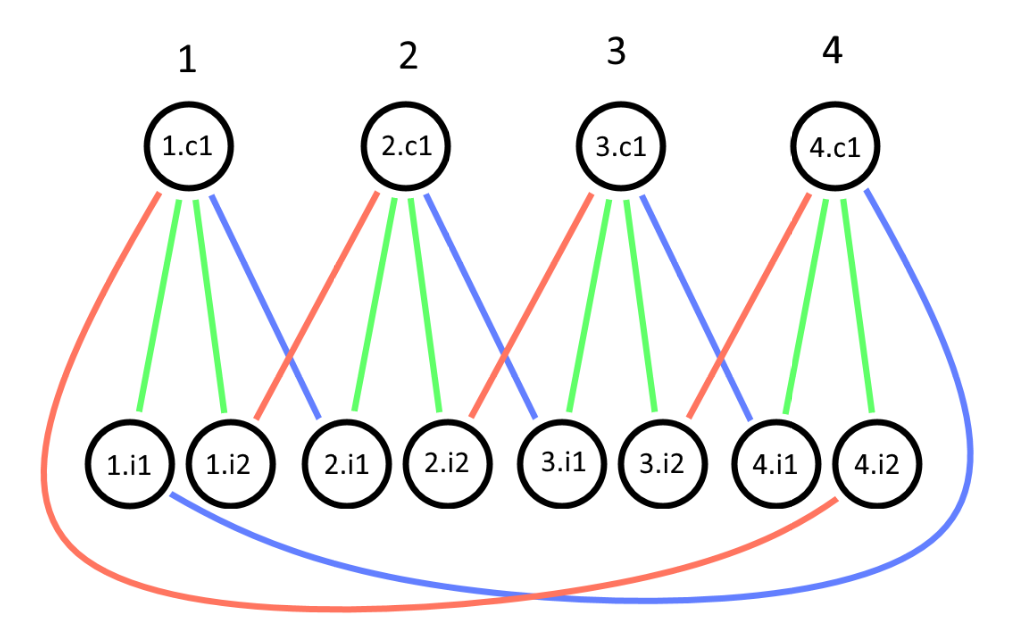
\includegraphics[scale=0.4]{Fig_1.png}
  \caption{ Граф с регулярной структурой. Компоненты пронумерованы от 1 до 4. Вершины помечены в формате \{номер компоненты\}.\{i, если вершина информационная, с, если проверочная\}\{номер вершины\} }\label{image:1}
\end{figure}

При анализе таких графов можно опустить параметр $K$, считая его достаточно большим, а затем при использовании подобрать его исходя из практических требований к размеру графа. Поэтому далее будем говорить о том, что регулярный граф задаётся тройкой $\langle c, i, f \rangle$.

\subsection{Упрощённое представление графов с\\ регулярной структурой}

Тройку $\langle c, i, f \rangle$, которой задаётся граф с регулярной структурой,\\ можно наглядно изобразить в виде графа, содержащего одну компоненту, в которой дуги проведены в соответствующие информационные вершины в этой же самой компоненте. Дуги следует пометить относительным номером компоненты, с которой она связана. Такой граф будем называть упрощённым представлением графа с регулярной структурой.

На рис. \ref{image:2} изображено подобное представление графа, соответствующего тройке $\langle 1, 2, f: f(1) = \{ (0, 1), (0, 2), (-1, 2), (1, 1) \} \rangle$

\begin{figure}[H]
  \centering
  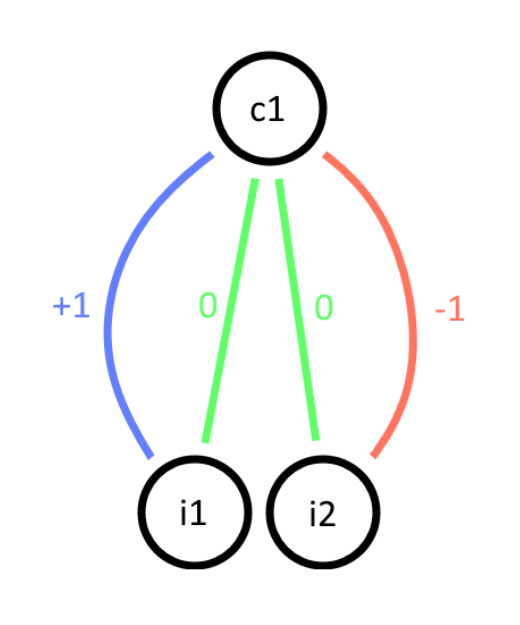
\includegraphics[scale=0.4]{Fig_2.png}
  \caption{ Упрощённое представление графа с регулярной структурой. }
  \label{image:2}
\end{figure}

\textbf{Замечание.}

Степени вершин графа с ргулярными структурами соответствуют количеству дуг, связанных с этими вершинами в упрощённом представлении графа.

\subsection{Поиск циклов в графах с регулярной\\ структурой}

Так как основная задача при построении таких графов ~--- контролировать длину минимального цикла, рассмотрим алгоритм поиска циклов в графе с регулярной структурой, заданном тройкой $\langle c, i, f \rangle$.

\textbf{Лемма 1.}

Если в графе с регулярными структурами есть цикл длины $t$, то через одну из проверочных вершин первой компоненты проходит цикл длины $t$.

\textbf{Доказательство.}

Пусть некий цикл $u: |u| = t$ проходит через компоненту проверочную вершину $j$ компоненты $d$. Из определения графа с регулярными компонентами, следует, что он изоморфен сам себе по отображению, циклически сдвигающему все вершины каждой $i$-той компоненты в $i + (d - 1) \pmod K$-тую компоненту. Такое отображение поставит в соответствие всем дугам, проходящим через $d$-тую компоненту дуги, проходящие через первую, а так как по определению это отображение ~--- изоморфизм, то оно поставит в соответствие циклу $u$ цикл $u': |u'| = |u|$, проходящий через $j$-тую проверочную вершину первой компоненты. Следовательно, существует цикл длины $t$, проходящий через $j$-тую проверочную вершину первой компоненты.

\qed

Из леммы 1 следует, что чтобы показать, что минимальный цикл в графе имеет длину $t$, достаточно убедиться, что через проверочные вершины одной компоненты не проходят циклы короче, чем $t$.

\textbf{Алгоритм 1.} 

Алгоритм принимает на вход номер начальной проверочной вершины, через которую должен проходить искомый цикл, и верхнее ограничение по длине искомого цикла.

В ходе работы алгоритма, вершины упрощённого представление графа с регулярной структурой помечаются числами. Пометка обозначает относительный номер компоненты, в которой достигнула данная вершина. Пометки разбиты на различные множества по поколению, которое обозначают длину найденного пути от заданной начальной вершины до данной вершины в данной компоненте.

Для каждой дуги $egde$ выражением $shift(edge)$ будем обозначать относительный сдвиг этой дуги, взятый с обратным знаком, если мы проходим по этой дуге от информационной дуги к проверочной.

Для каждой вершины $vertex$ выражением $sign(vertex)$ будем обозначать проверку, возвращающую $-1$, если вершина информационная и $1$, если вершина проверочная.

\begin{itemize}
\item Пометим начальную проверочную вершину числом $0$ в поколении $0$.
\item В цикле по поколениям $generation$ от $1$ до половины длины максимального цикла:
  \begin{itemize}
  \item Для всех пометок $label$ в поколении $generation - 1$:
    \begin{itemize}
    \item Вершину, которая помечена меткой $label$, обозначим $vertex$.
    \item Для всех дуг $edge$, с которыми соединена вершина, которая помечена меткой $label$:
      \begin{itemize}
      \item Число $label + shift(edge) * sign(vertex)$ обозначим $label'$
      \item Вершину, связанную с дугой $edge$ и не равную $vertex$, обозначим $vertex'$.
      \item Если $vertex'$ ещё не была помечена числом $label'$ ни в одном поколении ~--- пометить её этим числом в поколении $generation$.
      \item Если $vertex'$ была помечена помечена числом  $label'$ в поколении $generation$ ~--- сообщаем о том, что найден цикл длины $generation * 2$ и завершаем работу алгоритма.
      \end{itemize}
    \end{itemize}
  \end{itemize}
  \item Сообщаем о том, что цикл не найден и завершаем работу алгоритма.
\end{itemize}

\textbf{Замечание.}

Все вершины, помеченные в поколении $generation$, проверочные, если $generation$ ~-- нечётное и информационные, если $generaton$ ~--- чётное.
\\

\textbf{Теорема 1.}

Приведённый алгоритм находит кратчайший цикл, проходящий через заданную проверочную вершину $c$.

\textbf{Доказательство.}

Если существует кратчайший цикл длины $t$. Значит в этом цикле есть вершина $v$, до которой существует два пути длины $t / 2$ от вершины $c$. 

Покажем, что кратчайший путь от $c$ до $v$ имеет длину $t / 2$.  Предположим, что существует путь $path$, короче, чем $t / 2$. Если он не имеет общих дуг с одним из путей длины $t / 2$, то существует кратчайший цикл короче $t$, что противоречит предположению. Если он имеет общие дуги с одним из путей длины $t / 2$, то существует цикл, проходящий через вершину $c$ и через одну из общих дуг пути длины $t / 2$ и пути $path$, при этом не проходя через $v$. Так как $|path| + t / 2 < t$, то длина этого цикла меньше $t$, что противоречит предположению.

Покажем, что алгоритм помечает вершину $vertex$ меткой $label$ в поколении $generation$ тогда и только тогда, когда кратчайший путь от $c$ до вершины $vertex$ в компоненте $label$ раверн $generation$.

Доказательство проведём по индукции по  поколению $generation = 0, 1, ...$. 

\begin{itemize}
  \item В поколении $generation = 0$ существует только одна метка: ею помечена сама начальная вершина $c$, её значение равно $0$. 
  \item Пусть утверждение верно для всех поколений $generation <= k - 1$.
  \item Вершина $v$ будет отмечена меткой $l$ в поколении $generation = k$, если:
  \begin{itemize} 
    \item Она ещё не была отмечена меткой $l$ в предыдущих поколениях. То есть, если не найден более короткий путь до вершины $v$ в компоненте $l$, 
    \item В поколении $generation = k - 1$ отмечена меткой $l - s$ вершина $v'$, которая связана c $v$ дугой $edge$, причём $s = shift(egde) * sign(v)$. То есть, $v$ в компоненте связана дугой с вершиной в компоненте $v'$ в компоненте $l - s$, кратчайший путь до которой имеет длину $k - 1$, $shift(edge)$ равняется номеру компоненты, в которой находится информацинная вершина дуги $edge$, относительно компоненты, в которой находится проверочная вершина дуги $edge$, поэтому когда нужно узнать номер компоненты относительно информационной вершины, значение $shift(edge)$ надо брать с обратным знаком.
  \end{itemize}
  То есть, если длина кратчайшего пути до вершины $v$ в компоненте $l$ равна $k$.
\end{itemize}

Алгоритм завершается, если существуют два пути одинаковой длины до какой-то вершины. Так как при длине кратчайшего цикла $t$ есть как минимум два различных пути длины $t /2$ до вершины $v$, принадлежащей этому циклу, а путей короче до неё не существует, алгоритм завершится, найдя кратчайший цикл.

\qed

На рис. \ref{image:3} изображён пример работы алгоритма. Для удобства поколения пометок подписаны и обозначены цветами. Нулевое поколение ~--- синим, первое ~--- зелёным, второе ~--- голубым, третье ~--- розовым, четвёртое ~--- жёлтым. Совпадающие метки в четвёртом поколении обведены красными рамками. 

В нулевом поколении существует только одна метка ~--- вершина $c1$ помечена нулём. В первом поколении алгоритм помечает вершину $i1$ числами $0$ и $2$, прийдя по дугам со сдвигами $0$ и $2$ соответственно, аналогичным образом вершина $i2$ помечена числами $0$ и $3$. Во втором поколении вершина $c1$ помечается числами $-2$ и $-3$, когда алгоритм проходит через дуги со сдвигами $2$ и $3$ от нулевых пометок на информационных вершинах, так же $2$ и $3$, когда алгоритм проходит через дуги с нулевым сдвигом от меток $2$ и $3$ соотвественно. Другое метки не создаются, потому что их значение должно быть нулевым, однако вершина $c1$ уже помечена нулём в прошлых поколениях. Аналогичным образом помечаются вершины в третьем и четвёртом поколениях. В четвёртом поколении возникли повторяющиеся метки, поэтому алгоритм сигнализирует о найдённом цикле длины $8$.

\begin{figure}[H]
  \centering
  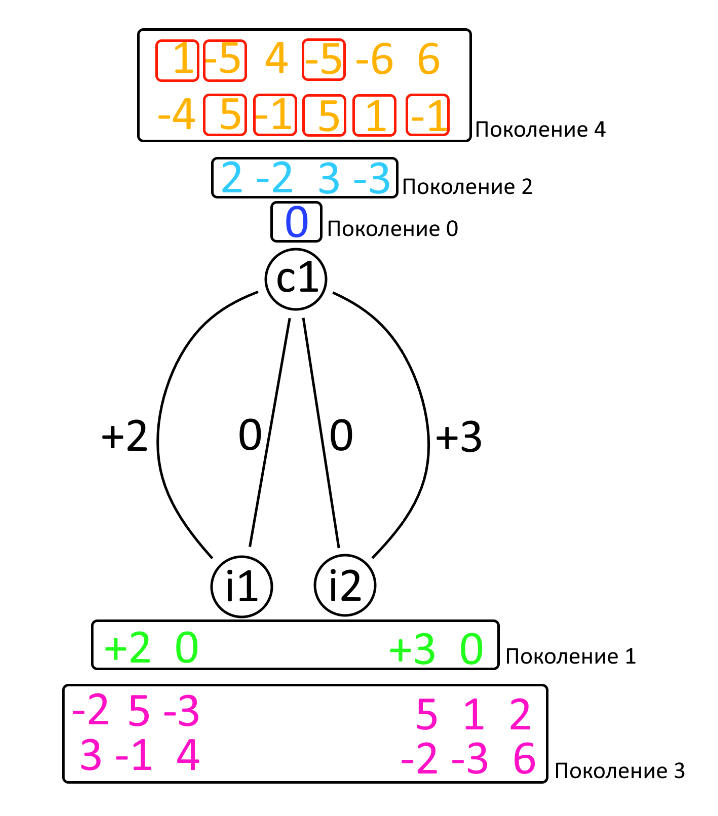
\includegraphics[scale=0.4]{Fig_3.png}
  \caption{ Пример работы алгоритма поиска циклов. }
  \label{image:3}
\end{figure}

Алгоритм легко доработать так, чтобы он возвращал список вершин, из которых состоит цикл. Для этого следует к меткам добавить ссылку на родительскую метку и затем, когда цикл найден, вернуться по ссылкам назад, собирая список вершин. На рис. \ref{image:4} изображён один из циклов, найденных в результате работы алгоритма. 

\begin{figure}[H]
  \centering
  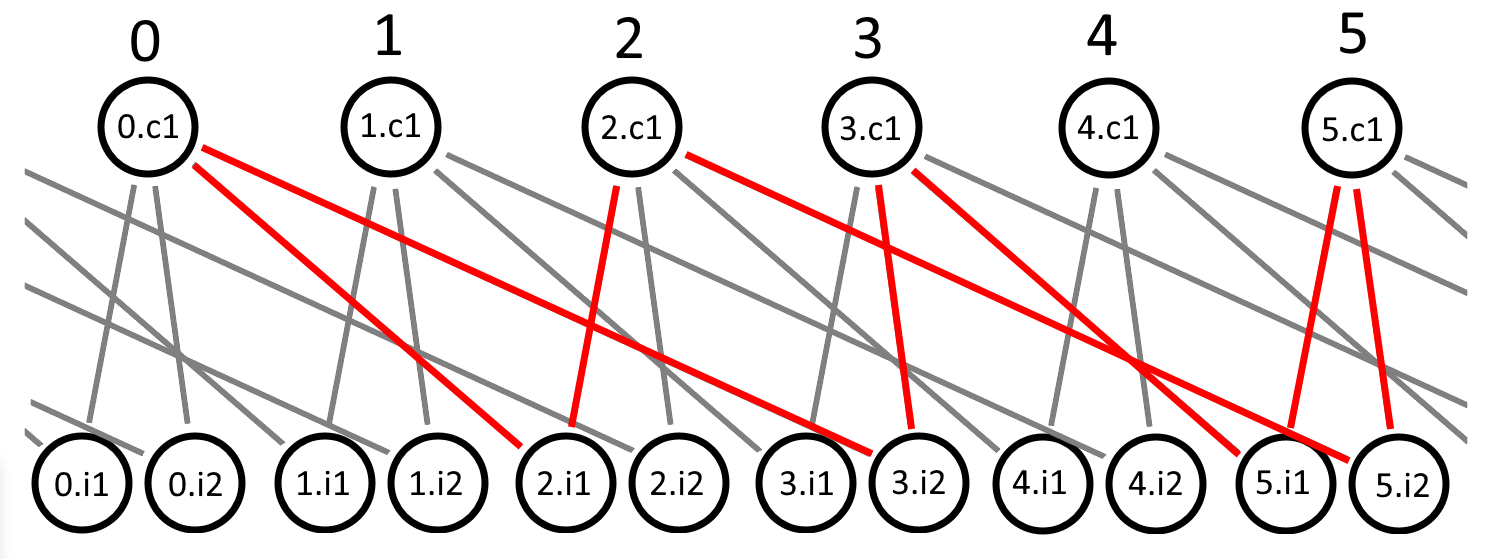
\includegraphics[scale=0.4]{Fig_4.png}
  \caption{ Пример цикла, найденного алгоритмом поиска циклов. }
  \label{image:4}
\end{figure}

На рис. \ref{image:5} изображён пример работы алгоритма на графе, дуги которого имеют неизвестные сдвиги, обозначенные буквами $a$, $b$ и $c$. Видно, что вне зависимости от значений переменных найден цикл-шестёрка.
 
\begin{figure}[H]
  \centering
  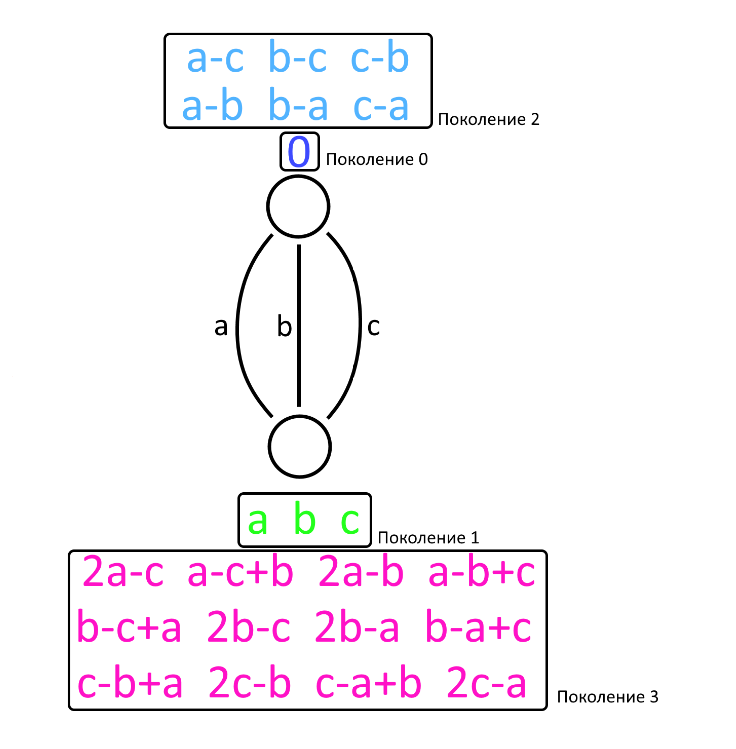
\includegraphics[scale=0.4]{Fig_5.png}
  \caption{ Пример поиска цикла на графе с неизвестными сдвигами. }
  \label{image:5}
\end{figure}

\textbf{Замечание.}

(3,n)-регулярные графы с регулярными структурами и обхватом\\ больше шести нельзя построить, если в компоненте только одна проверочная вершина, так как всякий такой граф будет содержать циклы-шестёрки, проходящие через первую информационную вершину.

%=======================

\section{Построение графа с заданным минимальным\\ циклом.}

\textbf{Алгоритм 2.}

На вход алгоритм получает число $t$ ~--- требуемый обхват графа и граф с регулярными структурами, заданный тройкой $\langle c, i, f \rangle$, где относительные сдвиги дуг, задаваемые $f$ неизвестны и обозначены $x_1, ..., x_e$.  

\begin{itemize}
\item Длину максимального допустимого цикла $t - 2$ обозначим $c$.
\item Инициализируем множество $I$.
\item Для каждой проверочной вершины $c$ компоненты графа:
\begin{itemize}
  \item Выполним алгоритм поиска циклов, с начальной вершиной $c$ и заданным максимальным допустимым циклом $c$.
  \item Если алгоритм нашёл цикл, то для заданной структуры компонентов нельзя построить граф с заданным обхватом.
  \item Добавляем в систему $I$ все неравенств вида $a \neq b$, где $a$ и $b$ ~--- это все различные метки на вершине $v$ в поколении $g$ $\forall v, g$
\end{itemize}
\item Составляем систему из всех неравенств,содержащихся в множестве $I$.
\item Находим решение $\alpha_1, ..., \alpha_e$ получившейся системы неравенств.
\item Возвращаем граф, заданный тройкой $\langle c, i, f \rangle$, где относительные сдвиги дуг, задаваемые $f$ имеют значения $\alpha_1, ..., \alpha_e$.
\end{itemize}

\textbf{Теорема 2.}

В результате корректного завершения работы алгоритма 2 получается граф с обхватом больше или равным требуемому.

\textbf{Доказательство.}

Алгоритм 2 в результате работы возвращает граф, заданный тройкой $\langle c, i, f \rangle$, где относительные сдвиги дуг, задаваемые $f$ имеют значения $\alpha_1, ..., \alpha_e$.

Для всех проверочных вершин компоненты выполним алгоритм 1 для полученного графа, передав ему $t - 2$, как длину максимального искомого цикла. 

Предположим, что алгоритм 1 завершил работу с сообщением о том, что обнаружен цикл, так как пометки на вершине $v$ в поколении $g$ совпали. Однако система неравенств, составленная алгоритмом 2 требует, чтобы все пометки на одной вершине в одном поколении различались. Возникает противоречие, следовательно в графе нет циклов с длиной меньше или равной $t - 2$, следовательно обхват графа равен $t$.

\qed

\textbf{Замечание.}

При использовании алгоритма 2 удобно в качестве пометок использовать вместо сумм вида $a_1 x_1 + a_2 x_2 + ... + a_e x_e$ кортежи вида $(a_1, a_2, ..., a_e)$. Неравенство вида $a_1 x_1 + ... + z_e x_e \neq b_1 x_1 + ... + b_e x_e$ можно записывать в виде кортежа $(a_1 - b_1, ..., a_e - b_e)$. Такой кортеж можно домножать на константу, что эквивалентно домножению на константу обеих сторон неравенства. 

\begin{figure}[H]
  \centering
  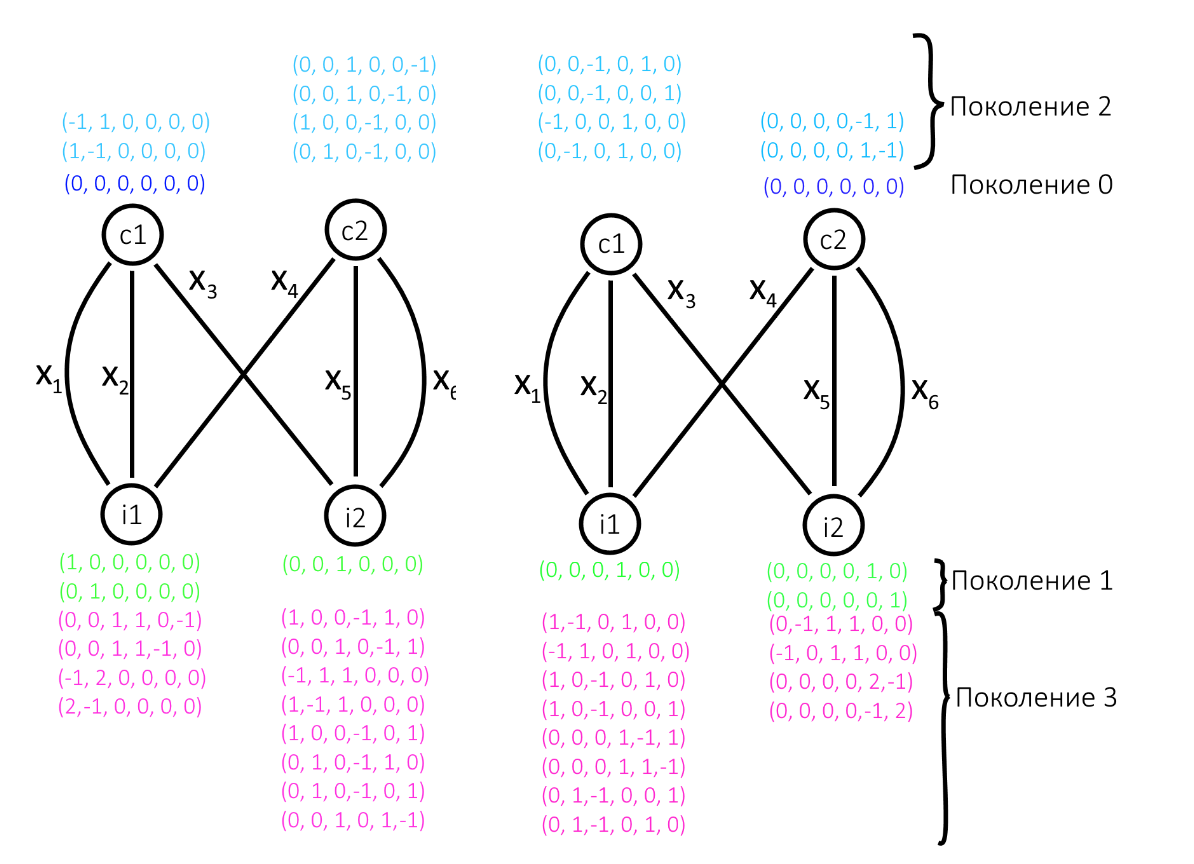
\includegraphics[scale=0.5]{Fig_6.png}
  \caption{ Первый этап работе алгоритма 2. }
  \label{image:6}
\end{figure}

На рис. \ref{image:6} изображены этапы работы алгоритма 2, связанные с поиском циклов с неизвестными относительнми сдвигами дуг, c требуемым обхватом 8, для графа с регулярными структурами, заданного тройкой $ \langle 2; 2; f\rangle $, где 
$$
  \begin{array}{ll}
    f(1) = \{ (x1, 1), (x2, 1), (x3, 2) \}\\
    f(2) = \{ (x4, 1), (x5, 2), (x6, 2) \}\\
  \end{array}
$$

Выполняется четыре итерации поиска циклов в общем виде для первой и второй проверочных вершин. Алгоритм не нашёл одинаковых кортежей в множествах пометок с одинаковой вершиной и поколением, значит, алгоритм продолжит поиск графа с обхватом 8.

Система неравенств (\ref{eqs:0}), получена для меток поколения $3$ на вершине $i2$, при поиске циклов, с начальной вершиной $c2$. Система \ref{eqs:1} ~--- она же, но записанная в матричной форме.

\begin{equation}
    \centering
    \left\{
        \begin{array}{ll}
            x_1 \neq x_2\\
            -x_2 + x_3 + x_4 \neq 2 x_5 - x_6\\
            -x_2 + x_3 + x_4 \neq -x_5 + 2 x_6\\
            -x_1 + x_3 + x_4 \neq 2 x_5 - x_6\\
            -x_1 + x_3 + x_4 \neq -x_5 + 2 x_6\\
            x_5 \neq x_6\\
        \end{array}
    \right.
    \label{eqs:0}
\end{equation}

\begin{equation}
    \centering
    \left(
        \begin{array}{ll}
            \ \ 1,-1,\ \ 0,\ \ 0,\ \ 0,\ \ 0\\
            \ \ 0,-1,\ \ 1,\ \ 1,-2,\ \ 1\\
            \ \ 0,-1,\ \ 1,\ \ 1,\ \ 1,-2\\
            -1,\ \ 0,\ \ 1,\ \ 1,-2,\ \ 1\\
            -1,\ \ 0,\ \ 1,\ \ 1,\ \ 1,-2\\
            \ \ 0,\ \ 0,\ \ 0,\ \ 0,\ \ 1,-1\\
        \end{array}
    \right)
    \label{eqs:1}
\end{equation}

Система неравенств (\ref{eqs:2}) получена для всех меток всех поколений для всех начальных вершин поиска циклов. Неравенства упрощены, повторения убраны.

\begin{figure}[H]
  \centering
  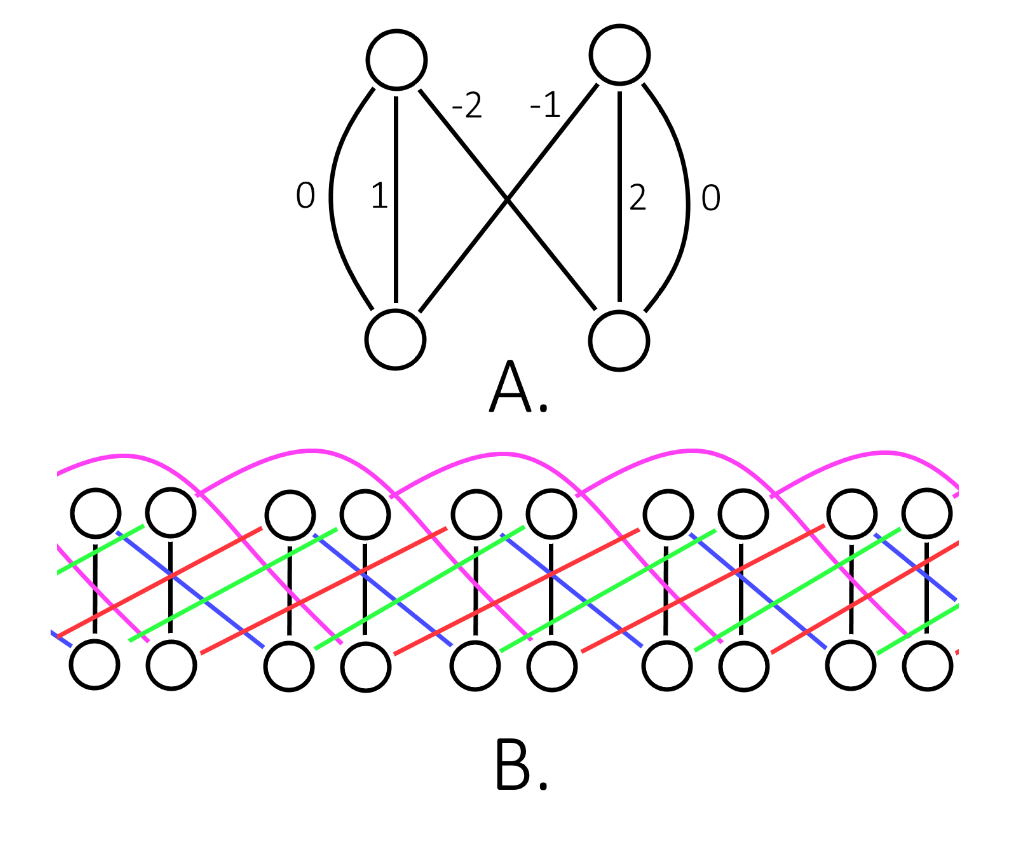
\includegraphics[scale=0.4]{Fig_7.png}
  \caption{ Граф полученный в результате работы алгоритма. A) В упрощённом представлении. B) В обычном представлении. }
  \label{image:7}
\end{figure}

Примером решения этой системы неравенств является кортеж $(0, 1,\\ -2, -1, 2, 0)$. Если подставить это решение в каждое неравнество, получится число отличное от нуля. Граф, заданный этим решением изображён на рис. \ref{image:7}.

\begin{equation}
  \centering
    \left(
      \begin{array}{ll}
        (1,-1,\ \ 0,\ \ 0,\ \ 0,\ \ 0)\\
        (0,\ \ 1,-1,-1,\ \ 0,\ \ 1)\\
        (0,\ \ 1,-1,-1,\ \ 1,\ \ 0)\\
        (1,\ \ 0,-1,-1,\ \ 0,\ \ 1)\\
        (1,\ \ 0,-1,-1,\ \ 1,\ \ 0)\\
        (0,\ \ 0,\ \ 0,\ \ 0,\ \ 1,-1)\\
        (1,\ \ 0,-1,-1,-1,\ \ 2)\\
        (1,-1,\ \ 0,\ \ 0,-1,\ \ 1)\\
        (2,-1,-1,-1,\ \ 0,\ \ 1)\\
        (1,-1,\ \ 0,\ \ 0,\ \ 1,-1)\\
        (2,-1,-1,-1,\ \ 1,\ \ 0)\\
        (1,\ \ 0,-1,-1,\ \ 2,-1)\\
        (0,\ \ 1,-1,-1,-1,\ \ 2)\\
        (1,-2,\ \ 1,\ \ 1,\ \ 0,-1)\\
        (1,-2,\ \ 1,\ \ 1,-1,\ \ 0)\\
        (0,\ \ 1,-1,-1,\ \ 2,-1)\\
      \end{array}
    \right)
  \label{eqs:2}
\end{equation}

 %=======================

\section{Решение систем неравенств}

\textbf{Алгоритм 3.}

Данный алгоритм можно использовать для поиска решения системы неравенств вида (\ref{eqs:example}).

\begin{equation}
    \centering
    \left\{
        \begin{array}{ll}
            a_{1,1} x_1 + ... + a_{1,e} x_e + b \neq 0\\
            ...\\
            a_{l,1} x_1 + ... + a_{l,1} x_e + b \neq 0\\
        \end{array}
    \right.
    \label{eqs:example}
\end{equation}

\begin{itemize}
    \item Найдём все неравенства  вида $a x_e + b = 0$. Обозначим множество таких неравенств $I$.
    \item Выберем число $v: v \neq -b/a \forall a x_e + b \in I$.
    \item Заменим во всех неравенствах $x_e$ на $v$ и выведем строку $x_e = v$.
    \item Если $e = 1$ ~--- завершим работу алгоритма.
    \item Запустим алгоритм для полученной системы неравнеств с $e - 1$ переменной.
\end{itemize}

\textbf{Теорема 3.}

Вывод алгоритма 3 является решением системы неравенств.

\textbf{Доказательство.}

Доказательство проведём по индукции по количеству переменных $e = 1, ...$.

\begin{itemize}
\item При $e = 1$ все неравенства имеют вид $a_j x_1 \neq b_j$. Результатом работы алгоритма будет число $v: v \neq -b_{j}/a_{j, 1} \forall j$. Такое число точно можно выбрать, так как неравенств конечное количество.
\item Предположим, что алгоритм корректно работает для систем с $e <= k - 1$ переменными.
\item Алгоритм заменит $x_e$ на $v: v \neq -b_{j}/a_{j, e}$ для всех неравенств вида $a_{j, e} x_e + b_j \neq 0$, такое число точно можно найти, так как неравенств конечное количество. В результате этой замены не возникнет неравенства вида $0 \neq 0$ по условию выбора $v$. Затем запустится алгоритм поиска решения неравенства с $e - 1$ переменными, который работает корректно по предположению индукции. 
\end{itemize}

\qed

\textbf{Замечание.}

Так как алгоритм 3 всегда завершается, мы можем говорить о том, что если в результате поиска в общем виде не обнаружил цикла с длиной меньше или равной $t$, то можно получить граф с обхватом $t$ заменой неизвестных сдвигов на соответствующие решения системы неравенств в рассмариваемом графе с регулярными структурами.

%=======================
\section{Метаграфы}

Серьёзный недостаток алгоритма 2 в том, что в процессе его работы используется система неравенств, которая растёт экспоненциально от длины цикла. Для уменьшения этой системы неравенств можно использовать метаграфы \cite{metagraphs}.

\subsection{Определение}

\textbf{Определение 9.}

\textsl{Метаграф} ~--- это двудольный граф, дугам которого поставлены в соответствие двоичные матрицы. Из метаграфа можно получить граф Таннера, если сопоставить каждой вершине набор из $K$ вершин, а каждой дуге ~--- набор дуг, построенный по соответствующей ей матрице размера $K \times K$. Такой процесс будем называть увеличением в $K$ раз. 

В качестве матриц в метаграфах будем использовать матрицы-\\-циркулянты, образованные вектором, содержащим одну единицу и нули. Тогда одной дуге метаграфа будет соответствовать ровно $K$ дуг. Группа таких матриц размера $K$ изоморфна $Z_K$, поэтому можно ставить дугам в соответствие целые числа, подразумевая соответствующие матрицы. Далее будем говорить только о таких метаграфах.

На рис. \ref{metagraph:1} изображён метаграф, с вершинами, помеченными числами, и результат увеличения его в 4 раза.

\subsection{Поиск циклов}

В работе \cite{metagraphs} показано, что цикл на метаграфе соответствует циклу на графе тогда и только тогда, когда сумма соответствующих дугам цикла чисел равна нулю по модулю $K$, причем числа дуг идущих от информационной вершины к проверочной должны быть взяты с обратным знаком.

\begin{figure}[H]
  \centering
  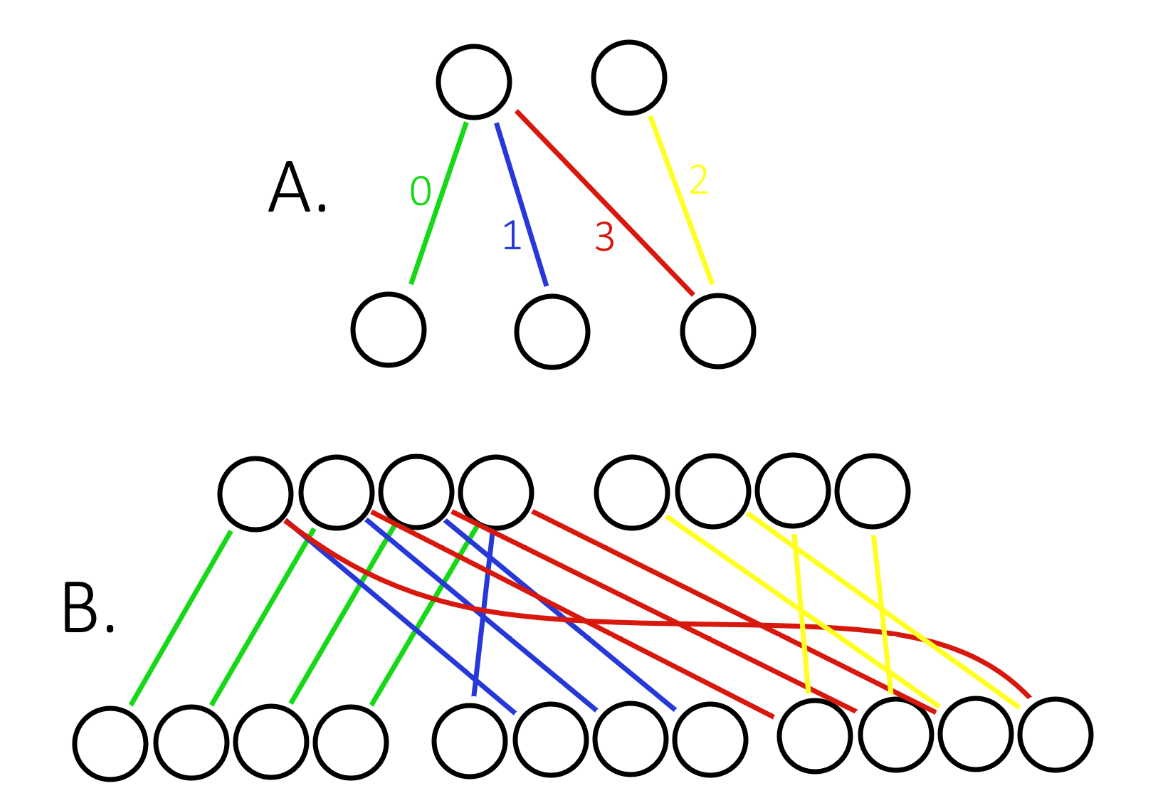
\includegraphics[scale=0.35]{Fig_8.png}
  \caption{ A) Метаграф. B) Результат увеличения метаграфа в 4 раза. }
  \label{metagraph:1}
\end{figure}

Можно модифицировать алгоритм 1 таким образом, чтобы он искал циклы на метаграфах с регулярными структурами. Для этого будем использовать в качестве пометок не числа, а пары $(a, b)$, где $a$ ~--- относительный сдвиг, который ранее составлял всю метку, а $b$ ~--- накопленная сумма соответствующих дугам метаграфа меток. Пары $(a_1, b_2)$ и $(a_2, b_2)$ считаются одинаковыми, если $a_1 = a_2$ и $b_1 \equiv b_2 \pmod K$. Когда к метке $(a, b)$ прибавляется сдвиг $s$ дуги, которой поставлено в соответствие число $c$, получается метка $(a + s, b + c \pmod K)$.

На рис. \ref{metagraph:2} изображена работа алгоритма поиска циклов на метаграфе. Длина минимального найденного цикла ~--- шесть. Причём если отбросить числа, сопоставленные дугам в метаграфе и работать с ним, как с обычным двудольным графом, обхват уменьшится до 4.

\textbf{Замечание.}

Если алгоритм поиска циклов в графах с регулярной структурой обнаружил цикл в графе неизвестными сдвигами, то цикл найдётся и в метаграфе с такой структурой и неизвестными числами, поставленными в соответствие дугам.

\begin{figure}[H]
  \centering
  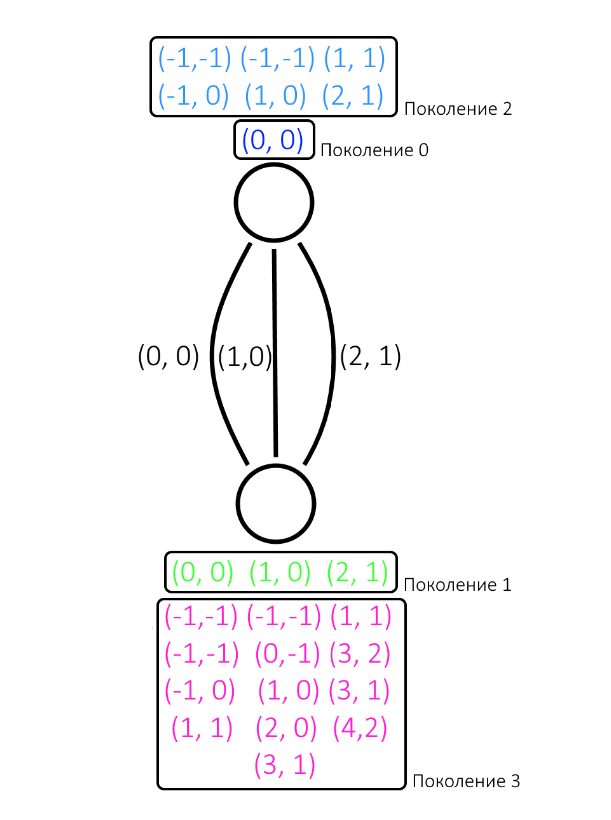
\includegraphics[scale=0.4]{Fig_9.png}
  \caption{ Работа алгоритма поиска циклов на метаграфе. }
  \label{metagraph:2}
\end{figure}

\subsection{Использование метаграфов в алгоритме\\ построения графа с заданным обхватом}

Применим алгоритм 2, используя алгоритм поиска циклов на метаграфе, вместо обычного алгоритма поиска циклов, обозначив сдвиги дуг $x_1, ..., x_e$, а числа, поставленные им в соответствие ~--- $y_1, ..., y_e$. В результате получится система неравенств вида (\ref{eqs:3}).

\begin{equation}
  \left\{
    \begin{array}{ll}
        \left[  
          \begin{array}{ll}
              a_{1,1} x_1 + ... + a_{1,e} x_e \neq 0 \\
              a_{1,1} y_1 + ... + a_{1,e} y_e \not\equiv 0 \pmod K \\
          \end{array}
        \right.\\
        ...\\
        \left[  
          \begin{array}{ll}
              a_{l,1} x_1 + ... + b_{l,e} x_e \neq 0 \\
              b_{l,1} y_1 + ... + b_{l,e} y_e \not\equiv 0 \pmod K \\
          \end{array}
        \right.\\
    \end{array}
  \right.
  \label{eqs:3}
\end{equation}

Устройство системы неравенств позволяет заранее выбрать числа, поставленные в соответствие дугам и избавить от части неравенств ещё на этапе генерации системы. Хорошими вариантами значений для таких чисел являются числа из последовательности Сидона \cite{sidon}.

%=======================
\newpage
\addcontentsline{toc}{section}{Заключение}
\section*{Заключение}

В данной работе были изучены графы с регулярной структурой, также для них разработано упрощённое представление. Доказано вспомогательное утверждение о поиске циклов в графе с регулярной структурой.

Разработаны следующте алгоритмы:

\begin{itemize}
  \item Алгоритм быстрого поиска цикла минимальной длины на графах с регулярной структурой, основанный на анализе упрощённого представления графа.
  \item Алгоритм построения графа с регулярной структурой с заданным обхватом.
  \item Вспомогательный алгоритм поиска решения системы неравенств определённого вида, возникающей в результате работы предыдущего алгоритма.
\end{itemize}

Приведены доказательства предложенных алгоритмов.

Разработан метод использования метагрфаов при построении графа с заданным обхватом.

%=======================
\newpage

\addcontentsline{toc}{section}{Литература}
\renewcommand{\refname}{\centering \textbf{Литература}}

\begin{thebibliography}{0}

\bibitem{zemor}
G. Zémor, On Expander Codes, IEEE Trans. on Information theory, IT-47
No 2, (2001) pp. 835–837.
  
\bibitem{johnson}
S.\,J. Johnson,
Introducing Low-Density Parity-Check Codes.
~-- University of Newcastle, Australia, 2006.

\bibitem{gallager}
R.\,G. Gallager,
Low-density parity-check codes
~-- IRE Transactions on Information Theory, 1962.

\bibitem{bruteforce}
Гурский С.\,С., Могилевская Н.\,С.
Задача генерации проверочных матриц ldpc-кодов.
~-- Ростов н/Д : Материалы конференции СИТО, 2021.

\bibitem{protographs}
J. Thorpe,
Low-density parity-check (LDPC) codes constructed from protographs.
~-- JPL, IPN Progress Rep., Aug. 2003, vol. 42–154.

\bibitem{metagraphs}
Арутюнов О.\,В.
Построение (m, n)-регулярных двудольных графов с наибольшим обхватом методом увеличения метаграфов.
~-- Ростов н/Д : Материалы конференции СИТО, 2021.

\bibitem{sidon}
J. Singer,
Perfect difference sets
~-- Brooklyn College, Brooklyn, N. Y, 1966.

\end{thebibliography}

\end{document}
% ----------------------------------------------------------------


\lstset{ %
language=C++,                 % выбор языка для подсветки (здесь это С++)
basicstyle=\small\sffamily, % размер и начертание шрифта для подсветки кода
numbers=left,               % где поставить нумерацию строк (слева\справа)
numberstyle=\tiny,           % размер шрифта для номеров строк
stepnumber=1,                   % размер шага между двумя номерами строк
numbersep=5pt,                % как далеко отстоят номера строк от подсвечиваемого кода
backgroundcolor=\color{white}, % цвет фона подсветки - используем \usepackage{color}
showspaces=false,            % показывать или нет пробелы специальными отступами
showstringspaces=false,      % показывать или нет пробелы в строках
showtabs=false,             % показывать или нет табуляцию в строках
frame=single,              % рисовать рамку вокруг кода
tabsize=2,                 % размер табуляции по умолчанию равен 2 пробелам
captionpos=t,              % позиция заголовка вверху [t] или внизу [b]
breaklines=true,           % автоматически переносить строки (да\нет)
breakatwhitespace=false, % переносить строки только если есть пробел
escapeinside={\%*}{*)}   % если нужно добавить комментарии в коде
extendedchars=true,
commentstyle=\color{mygreen},    % comment style
stringstyle=\bf,
commentstyle=\ttfamily\itshape,
keepspaces=true % пробелы между русскими буквами
aboveskip=3mm,
belowskip=3mm

}


\renewcommand\NAT@bibsetnum[1]{\settowidth\labelwidth{\@biblabel{#1}}%
   \setlength{\leftmargin}{\bibindent}\addtolength{\leftmargin}{\dimexpr\labelwidth+\labelsep\relax}%
   \setlength{\itemindent}{-\bibindent+\fivecharsapprox}%
   \setlength{\listparindent}{\itemindent}
\setlength{\itemsep}{\bibsep}\setlength{\parsep}{\z@}%
   \ifNAT@openbib
     \addtolength{\leftmargin}{\bibindent}%
     \setlength{\itemindent}{-\bibindent}%
     \setlength{\listparindent}{\itemindent}%
     \setlength{\parsep}{0pt}%
   \fi
}
\renewcommand{\thesection}{\arabic{section}.}
\renewcommand{\thesubsection}{\arabic{section}.\arabic{subsection}.}
